\documentclass[11pt]{article}
\usepackage{amsmath} 
\usepackage{graphicx}
\usepackage{subcaption}
\usepackage{sectsty}
\usepackage{amssymb}
 \usepackage{lipsum}
\usepackage{titlesec}
\usepackage{romannum}
\usepackage{enumitem}
\usepackage{mathtools}
\usepackage[super]{nth}
\usepackage{tikz}
\usepackage{listings}
\usepackage{pagecolor,lipsum}
\usepackage{color,soul}
\usepackage{xcolor}
\usepackage[T1]{fontenc}
\usepackage{textcomp}
\usepackage{float}
\definecolor{dkgreen}{rgb}{0,0.6,0}
\definecolor{gray}{rgb}{0.5,0.5,0.5}
\definecolor{mauve}{rgb}{0.58,0,0.82}
\definecolor{codegreen}{rgb}{0,0.6,0}
\definecolor{codegray}{rgb}{0.5,0.5,0.5}
\definecolor{codepurple}{rgb}{0.58,0,0.82}
\definecolor{backcolour}{rgb}{0.95,0.95,0.92}
\definecolor{orange}{RGB}{255,127,0}
\pagecolor{white}
\graphicspath{ {./images/} }

\lstdefinelanguage{JavaScript}{
  keywords={typeof, new, catch, function, return, null, catch, switch, var, if, in, while, do, else, case, break, let, log, const, console},
  keywordstyle=\color{blue}\bfseries,
  ndkeywords={class, export, boolean, throw, implements, import, this, true, false},
  ndkeywordstyle=\color{darkgray}\bfseries,
  identifierstyle=\color{black},
  sensitive=false,
  comment=[l]{//},
  morecomment=[s]{/*}{*/},
  commentstyle=\color{purple}\ttfamily,
  stringstyle=\color{red}\ttfamily,
  morestring=[b]',
  morestring=[b]"
}

\lstset{
   %frame = tb
   language=JavaScript,
   backgroundcolor=\color{backcolour},
   extendedchars=true,
   basicstyle=\small\ttfamily,
   showstringspaces=false,
   showspaces=false,
   numberstyle=\tiny\color{codegray},
   ndkeywordstyle=\color{codegreen}\bfseries,
   keywordstyle=\color{blue},
   commentstyle=\color{gray},
   stringstyle=\color{mauve},
   numbers=none,
   %numberstyle=\footnotesize,
   numbersep=9pt,
   tabsize=2,
   breaklines=true,
   showtabs=false,
   captionpos=b, 
   escapeinside={(*@}{@*)} 
}
\iffalse

\lstset{frame=tb,
  language=Javascript,
  aboveskip=3mm,
  belowskip=3mm,
  showstringspaces=false,
  columns=flexible,
  basicstyle={\small\ttfamily},
  numbers=left, %eller none
  numberstyle=\tiny\color{codegray},
  keywordstyle=\color{mauve},
  commentstyle=\color{gray},
  stringstyle=\color{orange},
  breaklines=false,
  breakatwhitespace=true,
  tabsize=3,
  escapeinside={(*@}{@*)}, 
 % backgroundcolor=\color{backcolour},  
}

\fi
\newcommand*\circled[1]{\tikz[baseline=(char.base)]{
            \node[shape=circle,draw,inner sep=2pt] (char) {#1};}}

\setlist[itemize,1]{leftmargin=\dimexpr 26pt-.5in}

\sectionfont{\fontsize{12}{15}\selectfont}
\title{Introduction to Programming with Javascript}
\author{Qitian Liao}
\date{Aug 3, 2020} 
\usepackage[left=2cm, right=2cm, top=2cm]{geometry}
%\setlength\parindent{0pt}

\DeclarePairedDelimiter\abs{\lvert}{\rvert}
\DeclarePairedDelimiter\norm{\lVert}{\rVert}

\begin{document}
\maketitle
\thispagestyle{empty}
\newpage
\tableofcontents
\thispagestyle{empty}
\cleardoublepage
\setcounter{page}{1}
\def\Arg{\mathop{\operator@font Arg}\nolimits}
%\newpage
\pagenumbering{arabic}
\titleformat*{\section}{\Large\bfseries}
\titleformat*{\subsection}{\large\bfseries}
\titleformat*{\subsubsection}{\normalsize\bfseries}
\titleformat*{\paragraph}{\large\bfseries}
\titleformat*{\subparagraph}{\large\bfseries}

%\titlespacing\section{0pt}{5pt plus 4pt minus 2pt}{5pt plus 2pt minus 2pt}
%\titlespacing\subsection{0pt}{10pt plus 4pt minus 2pt}{5pt plus 2pt minus 2pt}
%\titlespacing\subsubsection{0pt}{5pt plus 4pt minus 2pt}{5pt plus 2pt minus 2pt}
\newpage
\section{Introduction to Javascript}
\subsection{What is Javascript? }
Last year, millions of learners from our community started with JavaScript. Why? JavaScript is primarily known as the language of most modern web browsers, and its early quirks gave it a bit of a bad reputation. However, the language has continued to evolve and improve. JavaScript is a powerful, flexible, and fast programming language now being used for increasingly complex web development and beyond! \\
\newline
Since JavaScript remains at the core of web development, it’s often the first language learned by self-taught coders eager to learn and build. We’re excited for what you’ll be able to create with the JavaScript foundation you gain here. JavaScript powers the dynamic behavior on most websites, including this one. \\
\newline
In this lesson, you will learn introductory coding concepts including data types and built-in objects—essential knowledge for all aspiring developers. Make sure to take notes and pace yourself. This foundation will set you up for understanding the more complex concepts you’ll encounter later. 
\subsection{Console}
The console is a panel that displays important messages, like errors, for developers. Much of the work the computer does with our code is invisible to us by default. If we want to see things appear on our screen, we can print, or log, to our console directly. \\
\newline
In JavaScript, the \colorbox{lightgray}{console} keyword refers to an object, a collection of data and actions, that we can use in our code. Keywords are words that are built into the JavaScript language, so the computer will recognize them and treats them specially. \\
\newline
One action, or method, that is built into the \colorbox{lightgray}{console} object is the \colorbox{lightgray}{.log()} method. When we write \colorbox{lightgray}{console.log()} what we put inside the parentheses will get printed, or logged, to the console. It is going to be very useful for us to print values to the console, so we can see the work that we are doing.
\begin{lstlisting}
console.log(5); 
\end{lstlisting}
This example logs 5 to the console. The semicolon denotes the end of the line, or statement. Although in JavaScript your code will usually run as intended without a semicolon, we recommend learning the habit of ending each statement with a semicolon so you never leave one out in the few instances when they are required. \\
\newline
You’ll see later on that we can use \colorbox{lightgray}{console.log()} to print different kinds of data.
\subsection{Comments}
Programming is often highly collaborative. In addition, our own code can quickly become difficult to understand when we return to it. For these reasons, it’s often useful to leave notes in our code for other developers or ourselves.\\
\newline
As we write JavaScript, we can write comments in our code that the computer will ignore as our program runs. These comments exist just for human readers. Comments can explain what the code is doing, leave instructions for developers using the code, or add any other useful annotations. There are two types of code comments in JavaScript: 
\begin{enumerate}[leftmargin = *]
\item A \textit{single line comment} will comment out a single line and is denoted with two forward slashes \colorbox{lightgray}{//} preceding it.
\begin{lstlisting} 
// Prints 5 to the console
console.log(5);
\end{lstlisting}
You can also use a single line comment to comment after a line of code: 
\begin{lstlisting}
console.log(5);  // Prints 5 
\end{lstlisting}
\item A \textit{multi-line comment} will comment out multiple lines and is denoted with \colorbox{lightgray}{/*} to begin the comment, and \colorbox{lightgray}{*/} to end the comment.
\begin{lstlisting}
/*
This is all commented 
console.log(10);
None of this is going to run!
console.log(99);
*/
\end{lstlisting} 
You can also use this syntax to comment something out in the middle of a line of code: 
\begin{lstlisting} 
console.log(/*IGNORED!*/ 5);  // Still just prints 5 
\end{lstlisting}
\end{enumerate}
\subsection{Data Types}
\textit{Data types} are the classifications we give to the different kinds of data that we use in programming. In JavaScript, there are seven fundamental data types:
\begin{enumerate}[leftmargin = *]
\item \textit{Number}: Any number, including numbers with decimals: \colorbox{lightgray}{4}, \colorbox{lightgray}{8}, \colorbox{lightgray}{1516}, \colorbox{lightgray}{23.42}.
\item \textit{String}: Any grouping of characters on your keyboard (letters, numbers, spaces, symbols, etc.) surrounded by single quotes: \colorbox{lightgray}{` ... '} or double quotes \colorbox{lightgray}{`` ... "}. Though we prefer single quotes. Some people like to think of string as a fancy word for text. 
\item \textit{Boolean}: This data type only has two possible values— either \colorbox{lightgray}{true} or \colorbox{lightgray}{false} (without quotes). It’s helpful to think of booleans as on and off switches or as the answers to a “yes” or “no” question. 
\item \textit{Null}: This data type represents the intentional absence of a value, and is represented by the keyword \colorbox{lightgray}{null} (without quotes).
\item \textit{Undefined}: This data type is denoted by the keyword \colorbox{lightgray}{undefined} (without quotes). It also represents the absence of a value though it has a different use than \colorbox{lightgray}{null}.
\item \textit{Symbol}: A newer feature to the language, symbols are unique identifiers, useful in more complex coding. No need to worry about these for now.
\item \textit{Object}: Collections of related data.
\end{enumerate}
The first 6 of those types are considered \textit{primitive data types}. They are the most basic data types in the language. \textit{Objects} are more complex, and you will learn much more about them as you progress through JavaScript. At first, seven types may not seem like that many, but soon you will observe the world opens with possibilities once you start leveraging each one. As you learn more about objects, you’ll be able to create complex collections of data. But before we do that, let us first get comfortable with strings and numbers!
\begin{lstlisting}
console.log("Location of The Metropolitan: 2301 Durant Ave, Berkeley");
console.log(40);
\end{lstlisting}
In the example above, we first printed a string. Our string is not just a single word; it includes both capital and lowercase letters, spaces, and punctuation. Next, we printed the number 40, notice we did not use quotes.

\subsection{Arithmetic Operators}
Basic arithmetic often comes in handy when programming. An \textit{operator} is a character that performs a task in our code. JavaScript has several built-in in \textit{arithmetic operators}, that allow us to perform mathematical calculations on numbers. These include the following operators and their corresponding symbols:
\begin{enumerate}[leftmargin = *]
\item Add: \colorbox{lightgray}{$+$} 
\item Subtract: \colorbox{lightgray}{$-$}
\item Multiply: \colorbox{lightgray}{$*$}
\item Divide: \colorbox{lightgray}{$/$}
\item Remainder: \colorbox{lightgray}{$\%$}
\end{enumerate}
The first four work how you might guess:
\begin{lstlisting}
console.log(3 + 4); // Prints 7
console.log(5 - 1); // Prints 4
console.log(4 * 2); // Prints 8
console.log(9 / 3); // Prints 3
\end{lstlisting}
Note that when we \colorbox{lightgray}{console.log()} the computer will evaluate the expression inside the parentheses and print that result to the console. If we wanted to print the characters \colorbox{lightgray}{3 + 4}, we would wrap them in quotes and print them as a string.
\begin{lstlisting}
console.log(11 % 3); // Prints 2
console.log(12 % 3); // Prints 0 
\end{lstlisting}
The remainder operator, sometimes called \textit{modulo}, returns the number that remains after the right-hand number divides into the left-hand number as many times as it evenly can: \colorbox{lightgray}{11 \% 3} equals 2 because 3 fits into 11 three times, leaving 2 as the remainder.
\subsection{String Concatenation}
Operators are not just for numbers! When a \colorbox{lightgray}{$+$} operator is used on two strings, it appends the right string to the left string:
\begin{lstlisting}
console.log("hi" + "ya"); // Prints "hiya"
console.log("wo" + "ah"); // Prints "woah"
console.log("I love to " + "code."); // Prints "I love to code."
\end{lstlisting}
This process of appending one string to another is called \textit{concatenation}. Notice in the third example we had to make sure to include a space at the end of the first string. The computer will join the strings exactly, so we needed to make sure to include the space we wanted between the two strings.
\begin{lstlisting}
console.log("front " + "space"); // Prints "front space"
console.log("back" + " space"); // Prints "back space"
console.log("no" + "space"); // Prints "nospace"
console.log("middle" + " " + "space"); // Prints "middle space"
\end{lstlisting}
Just like with regular math, we can combine, or chain, our operations to get a final result:
\begin{lstlisting}
console.log("One" + ", " + "two" + ", " + "three!"); // Prints "One, two, three!"
\end{lstlisting}
\subsection{Properties}
When you introduce a new piece of data into a JavaScript program, the browser saves it as an instance of the data type. Every string instance has a property called \colorbox{lightgray}{length} that stores the number of characters in that string. You can retrieve property information by appending the string with a period and the property name:
\begin{lstlisting}
console.log("Hello".length); // Prints 5
\end{lstlisting}
The \colorbox{lightgray}{$.$} is another operator! We call it the dot operator. In the example above, the value saved to the \colorbox{lightgray}{length} property is retrieved from the instance of the string, \colorbox{lightgray}{'Hello'}. The program prints \colorbox{lightgray}{5} to the console, because \colorbox{lightgray}{Hello} has five characters in it.

\subsection{Methods}
Remember that methods are actions we can perform. JavaScript provides a number of string methods. We \textit{call}, or use, these methods by appending an instance with:
\begin{itemize}[leftmargin = *]
\item a period (the dot operator)
\item the name of the method
\item opening and closing parentheses
\end{itemize}
E.g. \colorbox{lightgray}{`example string'.methodName()}. \\
The syntax looks familiar. When we use \colorbox{lightgray}{console.log()} we’re calling the \colorbox{lightgray}{.log()} method on the \colorbox{lightgray}{console} object. Let us see \colorbox{lightgray}{console.log()} and some real string methods in action!
\begin{lstlisting}
console.log("hello".toUpperCase()); // Prints "HELLO"
console.log("Hey".startsWith("H")); // Prints true
\end{lstlisting}
Let’s look at each of the lines above: 
\begin{itemize}[leftmargin = *]
\item On the first line, the \colorbox{lightgray}{.toUpperCase()} method is called on the string instance \colorbox{lightgray}{`hello'}. The result is logged to the console. This method returns a string in all capital letters: \colorbox{lightgray}{`HELLO'}.
\item On the second line, the \colorbox{lightgray}{.startsWith()} method is called on the string instance \colorbox{lightgray}{`Hey'}. This method also accepts the character \colorbox{lightgray}{`H'} as an input, or argument, between the parentheses. Since the string \colorbox{lightgray}{`Hey'} does start with the letter \colorbox{lightgray}{`H'}, the method returns the boolean \colorbox{lightgray}{true}.
\end{itemize}
You can find a list of built-in string methods in the JavaScript documentation. \\
\underline{https://developer.mozilla.org/en-US/docs/Web/JavaScript/Reference/Global\_Objects/String}\\
Developers use documentation as a reference tool. It describes JavaScript’s keywords, methods, and syntax.
\subsection{Built-in Objects}
In addition to \colorbox{lightgray}{console}, there are other objects built into JavaScript. \\
\underline{https://developer.mozilla.org/en-US/docs/Web/JavaScript/Reference/Global\_Objects} \\
Down the line, you’ll build your own objects, but for now these “built-in” objects are full of useful functionality.
For example, if you wanted to perform more complex mathematical operations than arithmetic, JavaScript has the built-in \colorbox{lightgray}{Math} object. \\
\newline
The great thing about objects is that they have methods! Let’s call the \colorbox{lightgray}{.random()} method from the built-in \colorbox{lightgray}{Math} object:
\begin{lstlisting}
console.log(Math.random()); // Prints a random number between 0 and 1
\end{lstlisting}
In the example above, we called the \colorbox{lightgray}{.random()} method by appending the object name with the dot operator, the name of the method, and opening and closing parentheses. This method returns a random number between 0 and 1. \\
\newline
To generate a random number between 0 and 50, we could multiply this result by 50, like so:
\begin{lstlisting}
Math.random() * 50;
\end{lstlisting}
The example above will likely evaluate to a decimal. To ensure the answer is a whole number, we can take advantage of another useful \colorbox{lightgray}{Math} method called \colorbox{lightgray}{Math.floor()}. \\
\newline
\colorbox{lightgray}{Math.floor()} takes a decimal number, and rounds down to the nearest whole number. You can use \colorbox{lightgray}{Math.floor()} to round down a random number like this:
\begin{lstlisting}
Math.floor(Math.random() * 50);
\end{lstlisting}
In this case: 
\begin{enumerate}[leftmargin = *]
\item \colorbox{lightgray}{Math.random} generates a random number between 0 and 1.
\item We then multiply that number by \colorbox{lightgray}{50}, so now we have a number between 0 and 50.
\item Then, \colorbox{lightgray}{Math.floor()} rounds the number down to the nearest whole number.
\end{enumerate}
If you wanted to see the number printed to the terminal, you would still need to use a \colorbox{lightgray}{console.log()} statement:
\begin{lstlisting}
console.log(Math.floor(Math.random() * 50)); // Prints a random whole number between 0 and 50
\end{lstlisting}
To see all of the properties and methods on the Math object, take a look at the documentation here. \\
\underline{https://developer.mozilla.org/en-US/docs/Web/JavaScript/Reference/Global\_Objects/Math} \\
\underline{https://developer.mozilla.org/en-US/docs/Web/JavaScript/Reference/Global\_Objects/Number}
\subsection{Review}
Let us take one more glance at the concepts we just learned:
\begin{itemize}[leftmargin = *]
\item Data is printed, or logged, to the console, a panel that displays messages, with \colorbox{lightgray}{console.log()}.
\item We can write single-line comments with \colorbox{lightgray}{//} and multi-line comments between \colorbox{lightgray}{/*} and \colorbox{lightgray}{*/}.
\item There are 7 fundamental data types in JavaScript: strings, numbers, booleans, null, undefined, symbol, and object.
\item Numbers are any number without quotes: \colorbox{lightgray}{23.8879}
\item Strings are characters wrapped in single or double quotes: \colorbox{lightgray}{`Sample String'}
\item The built-in arithmetic operators include \colorbox{lightgray}{$+$}, \colorbox{lightgray}{$-$}, \colorbox{lightgray}{$*$}, \colorbox{lightgray}{$/$}, and \colorbox{lightgray}{$\%$}.
\item Objects, including instances of data types, can have properties, stored information. The properties are denoted with a \colorbox{lightgray}{.} after the name of the object, for example: \colorbox{lightgray}{`Hello'.length}.
\item Objects, including instances of data types, can have methods which perform actions. Methods are called by appending the object or instance with a period, the method name, and parentheses. For example: \colorbox{lightgray}{`hello'.toUpperCase()}.
\item We can access properties and methods by using the \colorbox{lightgray}{.}, dot operator.
\item Built-in objects, including \colorbox{lightgray}{Math}, are collections of methods and properties that JavaScript provides.
\end{itemize}

\newpage
\section{Variables}
\subsection{Variables}
In programming, a \textit{variable} is a container for a value. You can think of variables as little containers for information that live in a computer’s memory. Information stored in variables, such as a username, account number, or even personalized greeting can then be found in memory. \\
\newline
Variables also provide a way of labeling data with a descriptive name, so our programs can be understood more clearly by the reader and ourselves. \\
\newline
In short, variables label and store data in memory. There are only a few things you can do with variables: 
\begin{enumerate}[leftmargin = *]
\item Create a variable with a descriptive name.
\item Store or update information stored in a variable.
\item Reference or “get” information stored in a variable.
\end{enumerate}
It is important to distinguish that variables are not values; they contain values and represent them with a name. Later, we will cover how to use the \colorbox{lightgray}{var}, \colorbox{lightgray}{let}, and \colorbox{lightgray}{const} keywords to create variables.

\subsection{Create a Variable: var} 
There were a lot of changes introduced in the ES6 version of JavaScript in 2015. One of the biggest changes was two new keywords, \colorbox{lightgray}{let} and \colorbox{lightgray}{const}, to create, or declare, variables. Prior to the ES6, programmers could only use the \colorbox{lightgray}{var} keyword to declare variables.
\begin{lstlisting}
var myName = "Arya";
console.log(myName); // Output: Arya
\end{lstlisting}
Let’s consider the example above:
\begin{enumerate}[leftmargin = *]
\item \colorbox{lightgray}{var}, short for variable, is a JavaScript \textit{keyword} that creates, or \textit{declares}, a new variable.
\item \colorbox{lightgray}{myName} is the variable’s name. Capitalizing in this way is a standard convention in JavaScript called \textit{camel casing}. In camel casing you group words into one, the first word is lowercase, then every word that follows will have its first letter uppercased. (e.g. camelCaseEverything).
\item \colorbox{lightgray}{=} is the assignment operator. It assigns the value (\colorbox{lightgray}{`Arya'}) to the variable (\colorbox{lightgray}{myName}).
\item \colorbox{lightgray}{`Arya'} is the value assigned (\colorbox{lightgray}{=}) to the variable \colorbox{lightgray}{myName}. You can also say that the \colorbox{lightgray}{myName} variable is initialized with a value of \colorbox{lightgray}{`Arya'}.
\item After the variable is declared, the string value \colorbox{lightgray}{`Arya'} is printed to the console by referencing the variable name: \colorbox{lightgray}{console.log(myName)}.
\end{enumerate}
There are a few general rules for naming variables:
\begin{itemize}[leftmargin = *]
\item Variable names cannot start with numbers.
\item Variable names are case sensitive, so \colorbox{lightgray}{myName} and \colorbox{lightgray}{myname} would be different variables. It is bad practice to create two variables that have the same name using different cases.
\item Variable names cannot be the same as \textit{keywords}. For a comprehensive list of keywords check out MDN’s keyword documentation. \\
\underline{https://developer.mozilla.org/en-US/docs/Web/JavaScript/Reference/Statements/var}
\end{itemize}
Later, we will learn why ES6’s \colorbox{lightgray}{let} and \colorbox{lightgray}{const} are the preferred variable keywords by many programmers. Because there is still a ton of code written prior to ES6, it is helpful to be familiar with the pre-ES6 \colorbox{lightgray}{var} keyword. To learn more about \colorbox{lightgray}{var} and the quirks associated with it, check out the MDN var documentation. \\
\underline{https://developer.mozilla.org/en-US/docs/Web/JavaScript/Reference/Statements/var}

\subsection{Create a Variable: let}
As mentioned before, the \colorbox{lightgray}{let} keyword was introduced in ES6. The \colorbox{lightgray}{let} keyword signals that the variable can be reassigned a different value. Take a look at the example: 
\begin{lstlisting}
let meal = "Enchiladas";
console.log(meal); // Output: Enchiladas
meal = "Burrito";
console.log(meal); // Output: Burrito
\end{lstlisting}
Another concept that we should be aware of when using \colorbox{lightgray}{let} (and even \colorbox{lightgray}{var}) is that we can declare a variable without assigning the variable a value. In such a case, the variable will be automatically initialized with a value of \colorbox{lightgray}{undefined}:
\begin{lstlisting}
let price;
console.log(price); // Output: undefined
price = 350;
console.log(price); // Output: 350
\end{lstlisting}
Notice in the example above: 
\begin{itemize}[leftmargin = *]
\item If we don’t assign a value to a variable declared using the \colorbox{lightgray}{let} keyword, it automatically has a value of \colorbox{lightgray}{undefined}.
\item We can reassign the value of the variable.
\end{itemize}

\subsection{Create a Variable: const}
The \colorbox{lightgray}{const} keyword was also introduced in ES6, and is short for the word constant. Just like with \colorbox{lightgray}{var} and \colorbox{lightgray}{let} you can store any value in a \colorbox{lightgray}{const} variable. The way you declare a \colorbox{lightgray}{const} variable and assign a value to it follows the same structure as \colorbox{lightgray}{let} and \colorbox{lightgray}{var}. Take a look at the following example: 
\begin{lstlisting}
const myName = "Gilberto";
console.log(myName); // Output: Gilberto
\end{lstlisting}
However, a \colorbox{lightgray}{const} variable cannot be reassigned because it is constant. If you try to reassign a \colorbox{lightgray}{const} variable, you’ll get a \colorbox{lightgray}{TypeError}. \\
\newline
Constant variables must be assigned a value when declared. If you try to declare a \colorbox{lightgray}{const} variable without a value, you’ll get a \colorbox{lightgray}{SyntaxError}. \\
\newline
If you’re trying to decide between which keyword to use, \colorbox{lightgray}{let} or \colorbox{lightgray}{const}, think about whether you’ll need to reassign the variable later on. If you do need to reassign the variable use \colorbox{lightgray}{let}, otherwise, use \colorbox{lightgray}{const}.

\subsection{Mathematical Assignment Operators}
Let us consider how we can use variables and math operators to calculate new values and assign them to a variable. Check out the example below:
\begin{lstlisting}
let w = 4;
w = w + 1;
console.log(w); // Output: 5
\end{lstlisting}
In the example above, we created the variable \colorbox{lightgray}{w} with the number \colorbox{lightgray}{4} assigned to it. The following line, \colorbox{lightgray}{w = w + 1}, increases the value of \colorbox{lightgray}{w} from \colorbox{lightgray}{4} to \colorbox{lightgray}{5}. \\
\newline
Another way we could have reassigned \colorbox{lightgray}{w} after performing some mathematical operation on it is to use built-in \textit{mathematical assignment operators}. We could re-write the code above to be:
\begin{lstlisting}
let w = 4;
w += 1;
console.log(w); // Output: 5
\end{lstlisting}
In the second example, we used the \colorbox{lightgray}{+=} assignment operator to reassign \colorbox{lightgray}{w}. We’re performing the mathematical operation of the first operator \colorbox{lightgray}{+} using the number to the right, then reassigning \colorbox{lightgray}{w} to the computed value. \\
\newline
We also have access to other mathematical assignment operators: \colorbox{lightgray}{-=}, \colorbox{lightgray}{*=}, and \colorbox{lightgray}{/=} which work in a similar fashion. 
\begin{lstlisting}
let x = 20;
x -= 5; // Can be written as x = x - 5
console.log(x); // Output: 15

let y = 50;
y *= 2; // Can be written as y = y * 2
console.log(y); // Output: 100

let z = 8;
z /= 2; // Can be written as z = z / 2
console.log(z); // Output: 4 
\end{lstlisting}

\subsection{The Increment and Decrement Operator}
Other mathematical assignment operators include the increment operator (\colorbox{lightgray}{++}) and decrement operator (\colorbox{lightgray}{$--$}). The increment operator will increase the value of the variable by 1. The decrement operator will decrease the value of the variable by 1. For example:
\begin{lstlisting}
let a = 10;
a++;
console.log(a); // Output: 11
\end{lstlisting}
\begin{lstlisting}
let b = 20;
b--;
console.log(b); // Output: 19
\end{lstlisting}
Just like the previous mathematical assignment operators (\colorbox{lightgray}{+=}, \colorbox{lightgray}{$-$=}, \colorbox{lightgray}{*=}, \colorbox{lightgray}{/=}), the variable’s value is updated and assigned as the new value of that variable.

\subsection{String Concatenation with Variables}
Before we assigned strings to variables. Now, let us go over how to connect, or concatenate, strings in variables. The \colorbox{lightgray}{+} operator can be used to combine two string values even if those values are being stored in variables:
\begin{lstlisting}
let myPet = "armadillo";
console.log("I own a pet " + myPet + "."); // Output: "I own a pet armadillo."
\end{lstlisting}
In the example above, we assigned the value \colorbox{lightgray}{`armadillo'} to the \colorbox{lightgray}{myPet} variable. On the second line, the \colorbox{lightgray}{+} operator is used to combine three strings: \colorbox{lightgray}{`I own a pet'}, the value saved to \colorbox{lightgray}{myPet}, and \colorbox{lightgray}{`.'}. We log the result of this concatenation to the console as:
\begin{lstlisting}
I own a pet armadillo.
\end{lstlisting}

\subsection{String Interpolation}
In the ES6 version of JavaScript, we can insert, or \textit{interpolate}, variables into strings using \textit{template literals}. Check out the following example where a template literal is used to log strings together:
\textasciigrave
\begin{lstlisting}
const myPet = "armadillo";
console.log((*@\texttt{\textasciigrave}@*)I own a pet ${myPet}.(*@\texttt{\textasciigrave}@*)); // Output: I own a pet armadillo.
\end{lstlisting}
Notice that:
\begin{itemize}[leftmargin = *]
\item a template literal is wrapped by backticks \colorbox{lightgray}{\textasciigrave} (this key is usually located on the top of your keyboard, left of the \fbox{1} key).
\item Inside the template literal, you’ll see a placeholder, \colorbox{lightgray}{\$\{myPet\}}. The value of \colorbox{lightgray}{myPet} is inserted into the template literal.
\item When we interpolate \colorbox{lightgray}{\textasciigrave I own a pet \$\{myPet\}.\textasciigrave}, the output we print is the string: \colorbox{lightgray}{`I own a pet armadillo.'}
\end{itemize}
One of the biggest benefits to using template literals is the readability of the code. Using template literals, you can more easily tell what the new string will be. You also do not have to worry about escaping double quotes or single quotes. 

\subsection{typeof operator}
While writing code, it can be useful to keep track of the data types of the variables in your program. If you need to check the data type of a variable’s value, you can use the \colorbox{lightgray}{typeof} operator. The \colorbox{lightgray}{typeof} operator checks the value to its right and \textit{returns}, or passes back, a string of the data type. 
\begin{lstlisting}
const unknown1 = "foo";
console.log(typeof unknown1); // Output: string

const unknown2 = 10;
console.log(typeof unknown2); // Output: number

const unknown3 = true; 
console.log(typeof unknown3); // Output: boolean
\end{lstlisting}
Let us break down the first example. Since the value \colorbox{lightgray}{unknown1} is \colorbox{lightgray}{`foo'}, a string, \colorbox{lightgray}{typeof unknown1} will return \colorbox{lightgray}{`string'}.

\subsection{Review Variables}
Variables is a powerful concept you will use in all your future programming endeavors. Let us take one more glance at the concepts we just learned:
\begin{itemize}[leftmargin = *]
\item Variables hold reusable data in a program and associate it with a name. 
\item Variables are stored in memory.
\item The \colorbox{lightgray}{var} keyword is used in pre-ES6 versions of JS. 
\item \colorbox{lightgray}{let} is the preferred way to declare a variable when it can be reassigned, and \colorbox{lightgray}{const} is the preferred way to declare a variable with a constant value.
\item Variables that have not been initialized store the primitive data type \colorbox{lightgray}{undefined}. 
\item Mathematical assignment operators make it easy to calculate a new value and assign it to the same variable. 
\item The \colorbox{lightgray}{+} operator is used to concatenate strings including string values held in variables. 
\item In ES6, template literals use backticks \colorbox{lightgray}{\textasciigrave} and \colorbox{lightgray}{\$\{\}} to interpolate values into a string.
\item The \colorbox{lightgray}{typeof} keyword returns the data type (as a string) of a value.
\end{itemize}

\newpage
\section{Conditional Statements}
\subsection{What are Conditional Statements?}
In life, we make decisions based on circumstances. Think of an everyday decision as mundane as falling asleep — if we are tired, we go to bed, otherwise, we wake up and start our day. 
These if-else decisions can be modeled in code by creating \textit{conditional statements}. A conditional statement checks a specific condition(s) and performs a task based on the condition(s). \\
\newline
Now we will explore how programs make decisions by evaluating conditions and introduce logic into our code. We will cover the following concepts:
\begin{itemize}[leftmargin = *]
\item \colorbox{lightgray}{if}, \colorbox{lightgray}{else if}, and \colorbox{lightgray}{else} statements 
\item comparison operators
\item logical operators
\item truthy vs falsy values
\item ternary operators
\item \colorbox{lightgray}{switch} statement
\end{itemize}

\subsection{If Statement}
We often perform a task based on a condition. For example, if the weather is nice today, then we will go outside. If the alarm clock rings, then we will shut it off. If we are tired, then we will go to sleep. \\
\newline
In programming, we can also perform a task based on a condition using an \colorbox{lightgray}{if} statement:
\begin{lstlisting}
if (true) {
  console.log("This message will print!"); 
}
// Prints: This message will print!
\end{lstlisting}
Notice in the example above, we have an \colorbox{lightgray}{if} statement. The \colorbox{lightgray}{if} statement is composed of:
\begin{itemize}[leftmargin = *]
\item The \colorbox{lightgray}{if} keyword followed by a set of parentheses \colorbox{lightgray}{()} which is followed by a \textit{code block}, or \textit{block statement}, indicated by a set of curly braces \colorbox{lightgray}{\{\}}.
\item Inside the parentheses \colorbox{lightgray}{()}, a condition is provided that evaluates to \colorbox{lightgray}{true} or \colorbox{lightgray}{false}.
\item If the condition evaluates to \colorbox{lightgray}{true}, the code inside the curly braces \colorbox{lightgray}{\{\}} runs, or \textit{executes}.
\item If the condition evaluates to \colorbox{lightgray}{false}, the block will not execute.
\end{itemize}

\subsection{If...Else Statements}
In the previous chapter, we used an \colorbox{lightgray}{if} statement that checked a condition to decide whether or not to run a block of code. In many cases, we’ll have code we want to run if our condition evaluates to \colorbox{lightgray}{false}. \\
\newline
If we wanted to add some default behavior to the \colorbox{lightgray}{if} statement, we can add an \colorbox{lightgray}{else} statement to run a block of code when the condition evaluates to \colorbox{lightgray}{false}. Take a look at the inclusion of an \colorbox{lightgray}{else} statement: 
\begin{lstlisting}
if (false) {
  console.log("The code in this block will not run.");
} else {
  console.log("But the code in this block will!");
}

// Prints: But the code in this block will!
\end{lstlisting}
An \colorbox{lightgray}{else} statement must be paired with an \colorbox{lightgray}{if} statement, and together they are referred to as an \colorbox{lightgray}{if...else} statement. In the example above, the \colorbox{lightgray}{else} statement:
\begin{itemize}[leftmargin = *]
\item Uses the \colorbox{lightgray}{else} keyword following the code block of an \colorbox{lightgray}{if} statement.
\item Has a code block that is wrapped by a set of curly braces \colorbox{lightgray}{\{\}}.
\item The code inside the \colorbox{lightgray}{else} statement code block will execute when the \colorbox{lightgray}{if} statement’s condition evaluates to false.
\end{itemize}
\colorbox{lightgray}{if...else} statements allow us to automate solutions to yes-or-no questions, also known as binary decisions.

\subsection{Comparison Operators}
When writing conditional statements, sometimes we need to use different types of operators to compare values. These operators are called \textit{comparison operators}. Here is a list of some handy comparison operators and their syntax:
\begin{itemize}[leftmargin = *]
\item Less than: \colorbox{lightgray}{$<$}
\item Greater than: \colorbox{lightgray}{$>$}
\item Less than or equal to: \colorbox{lightgray}{$<$$=$}
\item Greater than or equal to: \colorbox{lightgray}{$>$$=$}
\item Is equal to: \colorbox{lightgray}{$=$$=$$=$}
\item Is not equal to: \colorbox{lightgray}{$!$$=$$=$}
\end{itemize}
Comparison operators compare the value on the left with the value on the right. For instance:
\begin{lstlisting}
10 < 12 // Evaluates to true
\end{lstlisting}
It can be helpful to think of comparison statements as questions. When the answer is “yes”, the statement evaluates to \colorbox{lightgray}{true}, and when the answer is “no”, the statement evaluates to \colorbox{lightgray}{false}. The code above would be asking: is 10 less than 12? Yes! So \colorbox{lightgray}{10 < 12} evaluates to \colorbox{lightgray}{true}. \\
\newline
We can also use comparison operators on different data types like strings:
\begin{lstlisting}
"apples" === "oranges" // false
\end{lstlisting}
In the example above, we’re using the identity operator (\colorbox{lightgray}{$=$$=$$=$}) to check if the string \colorbox{lightgray}{`apples'} is the same as the string \colorbox{lightgray}{`oranges'}. Since the two strings are not the same, the comparison statement evaluates to \colorbox{lightgray}{false}. \\
\newline
All comparison statements evaluate to either true or false and are made up of: 
\begin{itemize}[leftmargin = *]
\item Two values that will be compared.
\item An operator that separates the values and compares them accordingly (\colorbox{lightgray}{$>$}, \colorbox{lightgray}{$<$}, \colorbox{lightgray}{$<$$=$}, \colorbox{lightgray}{$>$$=$}, \colorbox{lightgray}{$=$$=$$=$} ,\colorbox{lightgray}{$!$$=$$=$}).
\end{itemize}
The difference between \colorbox{lightgray}{$=$$=$} and \colorbox{lightgray}{$=$$=$$=$} is that \colorbox{lightgray}{$=$$=$$=$}  is known as Identity / strict equality, meaning that the data types also must be equal. 
\begin{lstlisting}
console.log(1 == true) // output: true
console.log(1 === true) // output: false
\end{lstlisting}

\subsection{Logical Operators}
Working with conditionals means that we will be using booleans, \colorbox{lightgray}{true} or \colorbox{lightgray}{false} values. In JavaScript, there are operators that work with boolean values known as \textit{logical operators}. We can use logical operators to add more sophisticated logic to our conditionals. There are three logical operators: 
\begin{itemize}[leftmargin = *]
\item the and operator (\colorbox{lightgray}{$\&\&$})
\item the or operator (\colorbox{lightgray}{||})
\item the not operator, otherwise known as the bang operator (\colorbox{lightgray}{!}) 
\end{itemize}
When we use the \colorbox{lightgray}{$\&\&$} operator, we are checking that two things are true:
\begin{lstlisting}
if (stopLight === "green" && pedestrians === 0) {
  console.log("Go!");
} else {
  console.log("Stop");
}
\end{lstlisting}
When using the \colorbox{lightgray}{\&\&} operator, both conditions must evaluate to \colorbox{lightgray}{true} for the entire condition to evaluate to \colorbox{lightgray}{true} and execute. Otherwise, if either condition is \colorbox{lightgray}{false}, the \colorbox{lightgray}{\&\&} condition will evaluate to \colorbox{lightgray}{false} and the \colorbox{lightgray}{else} block will execute. \\
\newline
If we only care about either condition being true, we can use the \colorbox{lightgray}{||} operator:
\begin{lstlisting}
if (day === "Saturday" || day === "Sunday") {
  console.log("Enjoy the weekend!");
} else {
  console.log("Do some work.");
}
\end{lstlisting}
When using the \colorbox{lightgray}{||} operator, only one of the conditions must evaluate to \colorbox{lightgray}{true} for the overall statement to evaluate to \colorbox{lightgray}{true}. In the code example above, if either \colorbox{lightgray}{day $=$$=$$=$ `Saturday'} or \colorbox{lightgray}{day $=$$=$$=$ `Sunday'} evaluates to \colorbox{lightgray}{true} the \colorbox{lightgray}{if}‘s condition will evaluate to \colorbox{lightgray}{true} and its code block will execute. If the first condition in an \colorbox{lightgray}{||} statement evaluates to \colorbox{lightgray}{true}, the second condition will not even be checked. Only if \colorbox{lightgray}{day $=$$=$$=$ 'Saturday'} evaluates to \colorbox{lightgray}{false} will \colorbox{lightgray}{day $=$$=$$=$ 'Sunday'} be evaluated. The code in the \colorbox{lightgray}{else} statement above will execute only if both comparisons evaluate to \colorbox{lightgray}{false}. \\
\newline
The \colorbox{lightgray}{!} \textit{not operator reverses}, or \textit{negates}, the value of a boolean:
\begin{lstlisting}
let excited = true;
console.log(!excited); // Prints false

let sleepy = false;
console.log(!sleepy); // Prints true
\end{lstlisting}
Essentially, the \colorbox{lightgray}{!} operator will either take a \colorbox{lightgray}{true} value and pass back \colorbox{lightgray}{false}, or it will take a \colorbox{lightgray}{false} value and pass back \colorbox{lightgray}{true}. \\
\newline
Logical operators are often used in conditional statements to add another layer of logic to our code.

\subsection{Truthy and Falsy}
Let us consider how non-boolean data types, like strings or numbers, are evaluated when checked inside a condition. \\
\newline
Sometimes, you will want to check if a variable exists and you will not necessarily want it to equal a specific value — you’ll only check to see if the variable has been assigned a value. Here is an example:
\begin{lstlisting}
let myVariable = "I Exist!";

if (myVariable) {
   console.log(myVariable)
} else {
   console.log("The variable does not exist.")
}
\end{lstlisting}
The code block in the \colorbox{lightgray}{if} statement will run because \colorbox{lightgray}{myVariable} has a \textit{truthy} value; even though the value of \colorbox{lightgray}{myVariable} is not explicitly the value \colorbox{lightgray}{true}, when used in a boolean or conditional context, it evaluates to \colorbox{lightgray}{true} because it has been assigned a non-falsy value. \\
\newline
So which values are \textit{falsy}— or evaluate to \colorbox{lightgray}{false} when checked as a condition? The list of falsy values includes:
\begin{itemize}[leftmargin = *]
\item \colorbox{lightgray}{0}
\item Empty strings like \colorbox{lightgray}{``''} or \colorbox{lightgray}{`'}
\item \colorbox{lightgray}{null} which represent when there is no value at all
\item \colorbox{lightgray}{undefined} which represent when a declared variable lacks a value
\item \colorbox{lightgray}{NaN}, or Not a Number
\end{itemize}
Here’s an example with numbers: 
\begin{lstlisting}
let numberOfApples = 0;

if (numberOfApples){
   console.log("Let us eat apples!");
} else {
   console.log("No apples left!");
}

// Prints 'No apples left!'
\end{lstlisting}
The condition evaluates to \colorbox{lightgray}{false} because the value of the \colorbox{lightgray}{numberOfApples} is \colorbox{lightgray}{0}. Since \colorbox{lightgray}{0} is a falsy value, the code block in the \colorbox{lightgray}{else} statement will run.

\subsection{Truthy and Falsy Assignment}
Truthy and falsy evaluations open a world of short-hand possibilities. Say you have a website and want to take a user’s username to make a personalized greeting. Sometimes, the user does not have an account, making the \colorbox{lightgray}{username} variable falsy. The code below checks if \colorbox{lightgray}{username} is defined and assigns a default string if it is not:
\begin{lstlisting}
let defaultName;
if (username) {
  defaultName = username;
} else {
  defaultName = "Stranger";
}
\end{lstlisting}
If you combine your knowledge of logical operators you can use a short-hand for the code above. In a boolean condition, JavaScript assigns the truthy value to a variable if you use the \colorbox{lightgray}{||} operator in your assignment:
\begin{lstlisting}
let defaultName = username || "Stranger";
\end{lstlisting}
Because \colorbox{lightgray}{||} or statements check the left-hand condition first, the variable \colorbox{lightgray}{defaultName} will be assigned the actual value of \colorbox{lightgray}{username} if is truthy, and it will be assigned the value of \colorbox{lightgray}{`Stranger'} if \colorbox{lightgray}{username} is falsy. This concept is also referred to as \textit{short-circuit evaluation}.

\subsection{Ternary Operator}
In the spirit of using short-hand syntax, we can use a \textit{ternary operator} to simplify an \colorbox{lightgray}{if...else} statement. Take a look at the \colorbox{lightgray}{if...else} statement example: 
\begin{lstlisting}
let isNightTime = true;

if (isNightTime) {
  console.log("Turn on the lights!");
} else {
  console.log("Turn off the lights!");
}
\end{lstlisting}
We can use a \textit{ternary operator} to perform the same functionality:
\begin{lstlisting}
isNightTime ? console.log("Turn on the lights!") : console.log("Turn off the lights!");
\end{lstlisting}
In the example above:
\begin{itemize}[leftmargin = *]
\item The condition, \colorbox{lightgray}{isNightTime}, is provided before the \colorbox{lightgray}{?}.
\item Two expressions follow the \colorbox{lightgray}{?} and are separated by a colon \colorbox{lightgray}{:}.
\item If the condition evaluates to \colorbox{lightgray}{true}, the first expression executes.
\item If the condition evaluates to \colorbox{lightgray}{false}, the second expression executes.
\end{itemize}
Like \colorbox{lightgray}{if...else} statements, ternary operators can be used for conditions which evaluate to \colorbox{lightgray}{true} or \colorbox{lightgray}{false}.

\subsection{Else If Statements}
We can add more conditions to our \colorbox{lightgray}{if...else} with an \colorbox{lightgray}{else if} statement. The \colorbox{lightgray}{else if} statement allows for more than two possible outcomes. You can add as many \colorbox{lightgray}{else if} statements as you would like, to make more complex conditionals! \\
\newline
The \colorbox{lightgray}{else if} statement always comes after the \colorbox{lightgray}{if} statement and before the \colorbox{lightgray}{else} statement. The \colorbox{lightgray}{else if} statement also takes a condition. Let us take a look at the syntax:
\begin{lstlisting}
let stopLight = "yellow";

if (stopLight === "red") {
  console.log("Stop!");
} else if (stopLight === "yellow") {
  console.log("Slow down.");
} else if (stopLight === "green") {
  console.log("Go!");
} else {
  console.log("Caution, unknown!");
}
\end{lstlisting}
The \colorbox{lightgray}{else if} statements allow you to have multiple possible outcomes. \colorbox{lightgray}{if/else if/else} statements are read from top to bottom, so the first condition that evaluates to \colorbox{lightgray}{true} from the top to bottom is the block that gets executed. \\
\newline
In the example above, since \colorbox{lightgray}{stopLight $=$$=$$=$ `red'} evaluates to false and \colorbox{lightgray}{stopLight $=$$=$$=$ `yellow'} evaluates to \colorbox{lightgray}{true}, the code inside the first \colorbox{lightgray}{else if} statement is executed. The rest of the conditions are not evaluated. If none of the conditions evaluated to true, then the code in the \colorbox{lightgray}{else} statement would have executed.

\subsection{The switch keyword}
\colorbox{lightgray}{else if} statements are a great tool if we need to check multiple conditions. In programming, we often find ourselves needing to check multiple values and handling each of them differently. For example:
\begin{lstlisting}
let groceryItem = "papaya";

if (groceryItem === "tomato") {
  console.log("Tomatoes are $0.49");
} else if (groceryItem === "papaya"){
  console.log("Papayas are $1.29");
} else {
  console.log("Invalid item");
}
\end{lstlisting}
In the code above, we have a series of conditions checking for a value that matches a \colorbox{lightgray}{groceryItem} variable. Our code works fine, but imagine if we needed to check 100 different values. Having to write that many \colorbox{lightgray}{else if} statements sounds like a pain. \\
\newline
A \colorbox{lightgray}{switch} statement provides an alternative syntax that is easier to read and write. A \colorbox{lightgray}{switch} statement looks like this:
\begin{lstlisting}
let groceryItem = "papaya";

switch (groceryItem) {
  case "tomato":
    console.log("Tomatoes are $0.49");
    break;
  case "lime":
    console.log("Limes are $1.49");
    break;
  case "papaya":
    console.log("Papayas are $1.29");
    break;
  default:
    console.log("Invalid item");
    break;
}
// Prints "Papayas are $1.29"
\end{lstlisting}
\begin{itemize}[leftmargin = *]
\item The \colorbox{lightgray}{switch} keyword initiates the statement and is followed by \colorbox{lightgray}{( ... )}, which contains the value that each \colorbox{lightgray}{case} will compare. In the example, the value or expression of the \colorbox{lightgray}{switch} statement is \colorbox{lightgray}{groceryItem}.
\item Inside the block, \colorbox{lightgray}{\{ ... \}}, there are multiple \colorbox{lightgray}{case}s. The \colorbox{lightgray}{case} keyword checks if the expression matches the specified value that comes after it. The value following the first \colorbox{lightgray}{case} is \colorbox{lightgray}{`tomato'}. If the value of \colorbox{lightgray}{groceryItem} equalled \colorbox{lightgray}{`tomato'}, that \colorbox{lightgray}{case}'s \colorbox{lightgray}{console.log()} would run.
\item The value of \colorbox{lightgray}{groceryItem} is \colorbox{lightgray}{`papaya'}, so the third \colorbox{lightgray}{case} runs— \colorbox{lightgray}{Papayas are \$1.29} is logged to the console.
\item The \colorbox{lightgray}{break} keyword tells the computer to exit the block and not execute any more code or check any other cases inside the code block. Note: Without the \colorbox{lightgray}{break} keyword at the end of each case, the program would execute the code for all matching cases and the default code as well. This behavior is different from \colorbox{lightgray}{if}/\colorbox{lightgray}{else} conditional statements which execute only one block of code.
\item At the end of each \colorbox{lightgray}{switch} statement, there is a \colorbox{lightgray}{default} statement. If none of the \colorbox{lightgray}{case}s are true, then the code in the \colorbox{lightgray}{default} statement will run.
\end{itemize}

\subsection{Review}
Here are some of the major concepts for conditionals:
\begin{itemize}[leftmargin = *]
\item An \colorbox{lightgray}{if} statement checks a condition and will execute a task if that condition evaluates to \colorbox{lightgray}{true}.
\item \colorbox{lightgray}{if...else} statements make binary decisions and execute different code blocks based on a provided condition.
\item We can add more conditions using \colorbox{lightgray}{else if} statements.
\item Comparison operators, including \colorbox{lightgray}{$<$}, \colorbox{lightgray}{$>$}, \colorbox{lightgray}{$<$$=$}, \colorbox{lightgray}{$>$$=$}, \colorbox{lightgray}{$=$$=$$=$}, and \colorbox{lightgray}{$!$$=$$=$} can compare two values.
\item The logical and operator, \colorbox{lightgray}{\&\&}, or “and”, checks if both provided expressions are truthy.
\item The logical operator \colorbox{lightgray}{||}, or “or”, checks if either provided expression is truthy.
\item The bang operator, \colorbox{lightgray}{!}, switches the truthiness and falsiness of a value.
\item The ternary operator is shorthand to simplify concise \colorbox{lightgray}{if...else} statements.
\item A \colorbox{lightgray}{switch} statement can be used to simplify the process of writing multiple \colorbox{lightgray}{else if} statements. The \colorbox{lightgray}{break} keyword stops the remaining \colorbox{lightgray}{case}s from being checked and executed in a \colorbox{lightgray}{switch} statement.
\end{itemize}

\newpage
\section{Functions}
\subsection{What are Functions?}
When first learning how to calculate the area of a rectangle, there is a sequence of steps to calculate the correct answer:
\begin{enumerate}[leftmargin = *]
\item Measure the width of the rectangle.
\item Measure the height of the rectangle.
\item Multiply the width and height of the rectangle.
\end{enumerate}
With practice, you can calculate the area of the rectangle without being instructed with these three steps every time. We can calculate the area of one rectangle with the following code: 
\begin{lstlisting}
const width = 10;
const height = 6;
const area =  width * height;
console.log(area); // Output: 60
\end{lstlisting}
Imagine being asked to calculate the area of three different rectangles: 
\begin{lstlisting}
// Area of the first rectangle
const width1 = 10;
const height1 = 6;
const area1 =  width1 * height1;

// Area of the second rectangle
const width2 = 4;
const height2 = 9;
const area2 =  width2 * height2;

// Area of the third rectangle
const width3 = 10;
const height3 = 10;
const area3 =  width3 * height3;
\end{lstlisting}
In programming, we often use code to perform a specific task multiple times. Instead of rewriting the same code, we can group a block of code together and associate it with one task, then we can reuse that block of code whenever we need to perform the task again. We achieve this by creating a \textit{function}. A function is a reusable block of code that groups together a sequence of statements to perform a specific task. \\
\newline
Now, you will learn how to create and use functions, and how they can be used to create clearer and more concise code.

\subsection{Function Declarations} 
In JavaScript, there are many ways to create a function. One way to create a function is by using a \textit{function declaration}. Just like how a variable declaration binds a value to a variable name, a function declaration binds a function to a name, or an \textit{identifier}. Take a look at the anatomy of a function declaration below:
\begin{figure}[H]
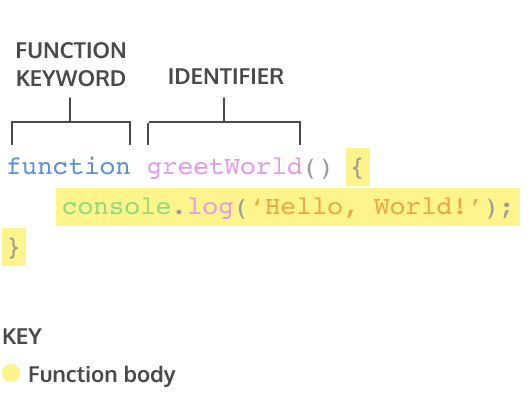
\includegraphics[scale = 0.8]{4_1}
\centering
\end{figure}
\noindent A function declaration consists of: 
\begin{itemize}[leftmargin = *]
\item The \colorbox{lightgray}{function} keyword.
\item The name of the function, or its identifier, followed by parentheses.
\item A function body, or the block of statements required to perform a specific task, enclosed in the function’s curly brackets, \colorbox{lightgray}{\{ \}}.
\end{itemize}
A function declaration is a function that is bound to an identifier, or name. In the next chapter, we will go over how to run the code inside the function body.
We should also be aware of the \textit{hoisting} feature in JavaScript which allows access to function declarations before they’re defined. Take a look at example of hoisting:
\begin{lstlisting}
console.log(greetWorld()); // Output: Hello, World!

function greetWorld() {
  console.log("Hello, World!");
}
\end{lstlisting}
Notice how hoisting allowed \colorbox{lightgray}{greetWorld()} to be called before the \colorbox{lightgray}{greetWorld()} function was defined! Since hoisting is not considered good practice, we simply want you to be aware of this feature.













\end{document}
